After successfully purifying the Quantum dots, the time for the deposition has come. We will now discuss used methods and then show the schematic for the steps taken in creating the device. 

\subsection{Glass contact cleaning}

To be sure that we can reduce a number of defects connected with dust and air pollution, the transparent glass contact needs to be cleaned. It it done with simple method using a strong detergent and solvent(in our case isopropanol). The glass is placed inside the holder and put in deionised water for rinsing. After few times, when the glass is clean it is then placed in the UV-ozone cleaning chamber. Inside, UV lamp either dissociates Oxygen into triplet and then it combines with $O_2$ generating ozone or with the higher wavelength dissociates $O_3$ and makes singlet oxygen in the process(it reacts with substrate surfaces strongly). It is a dry process, in which there is a low damage on the probes. 

\begin{figure}[ht]
\begin{subfigure}{.5\textwidth}
  \centering
  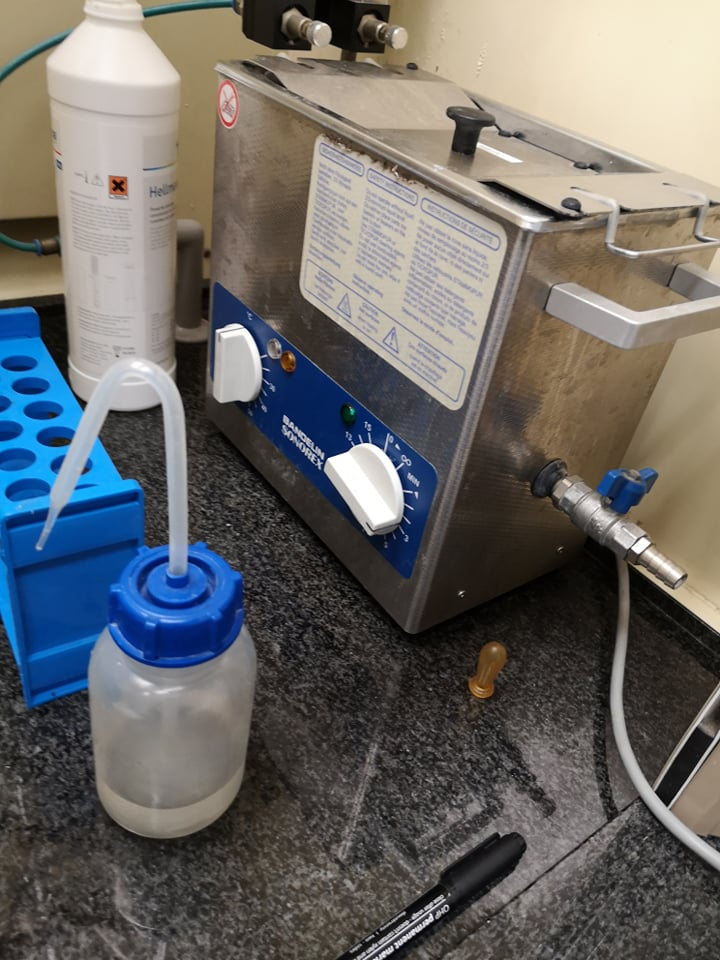
\includegraphics[width=.8\linewidth]{ch3/sono}  
  \caption{Ionized water cleaning equipment}
\end{subfigure}
\begin{subfigure}{.5\textwidth}
  \centering
  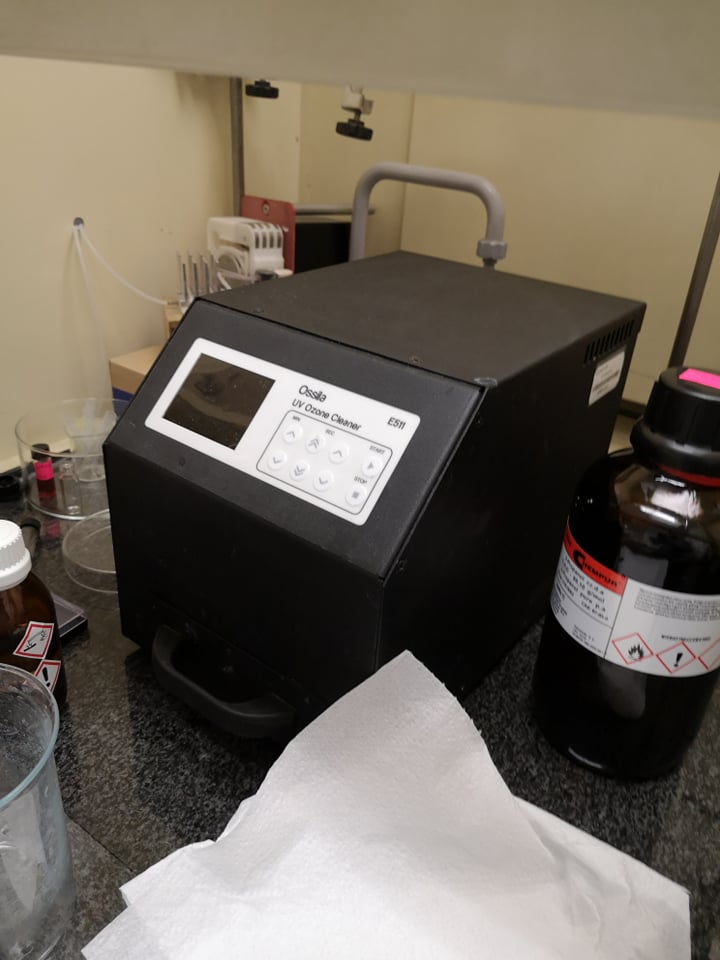
\includegraphics[width=.8\linewidth]{ch3/uv}  
  \caption{UV-ozone cleaning equipment}
\end{subfigure}
\caption{Cleaning methods environment}
\label{fig:clean}
\end{figure}

\subsection{Spin Coating}
To achieve an uniform deposition, the technique of applying a small amount of rotating material is used. The centrifugal force achieved with rotation allows to place the substrate only if it's possible to convey it on the surface for a longer period. Usually, as also in our case, the substrate can simultaneously evaporate during the process. With the angular speed, the thickness of a layer is parametrized, so higher the velocity, the thinner the layer. 


\begin{figure}[H]
\begin{subfigure}{.5\textwidth}
  \centering
  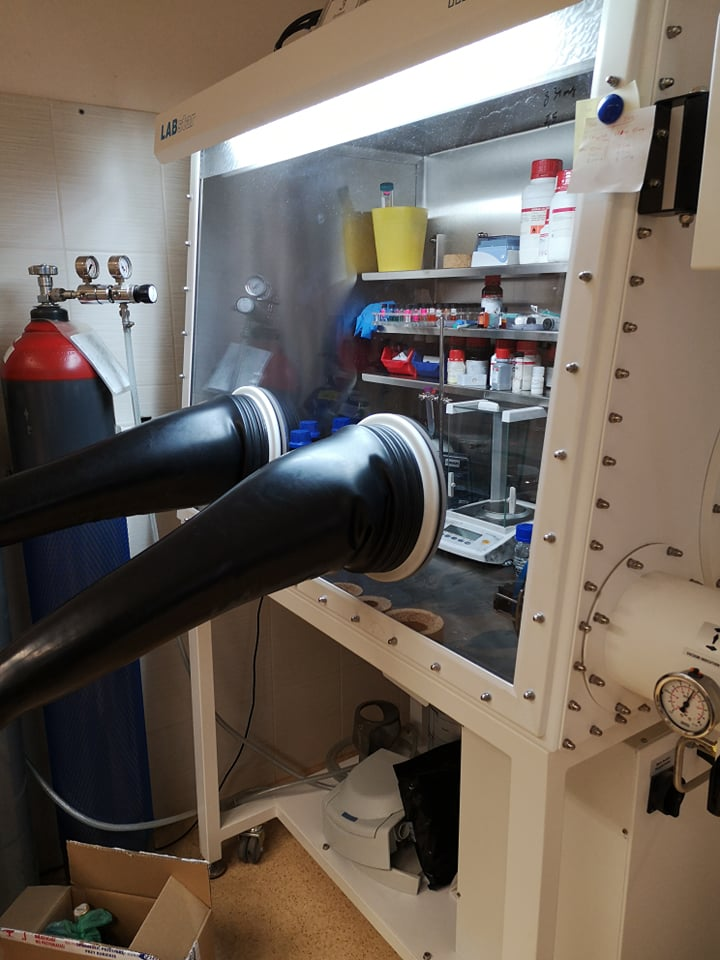
\includegraphics[width=.8\linewidth]{ch3/glovebox}  
  \caption{Glovebox used in the laboratory}
\end{subfigure}
\begin{subfigure}{.5\textwidth}
  \centering
  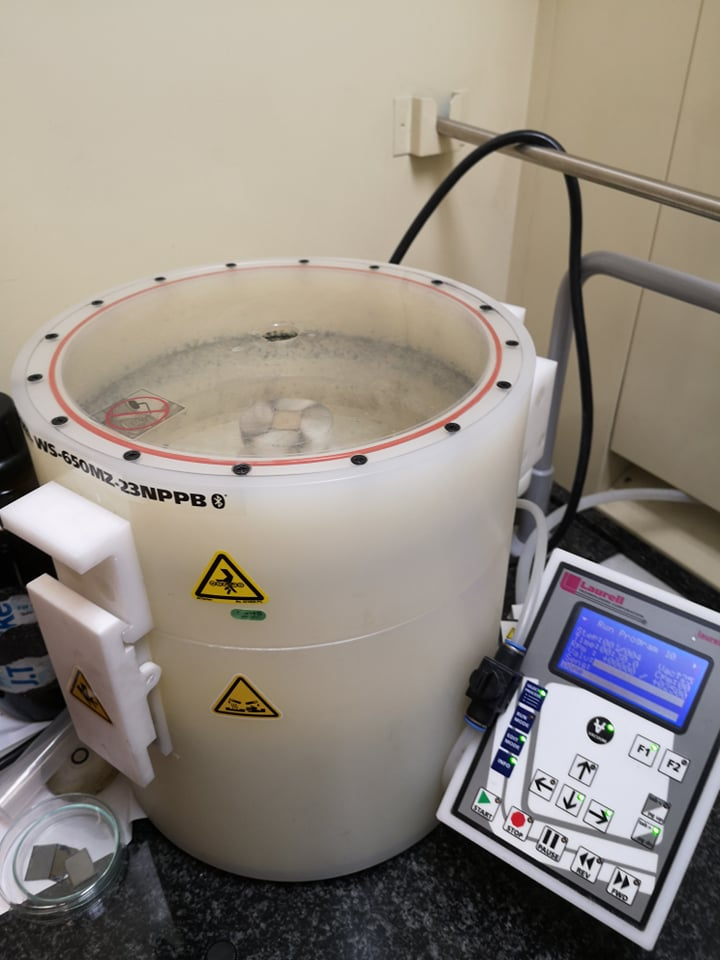
\includegraphics[width=.8\linewidth]{ch3/spincoater}  
  \caption{Spincoater used in the laboratory}
\end{subfigure}
\label{fig:gloves}
\caption{Laboratory equipment view}
\end{figure}

\subsection{Glovebox}

It has to be highlighted that some of the processes cannot be done with the contact of air. Therefore, a single machine called glovebox is used to overcome some of the task and to ensure even higher quality of the out-coming creation. Inside it, the inert atmosphere is made with using nitrogen so the items need to be inserted with vacuum pump.
\newpage
\subsection{Sputter deposition}

\begin{wrapfigure}{r}{0.401\textwidth}
\centering
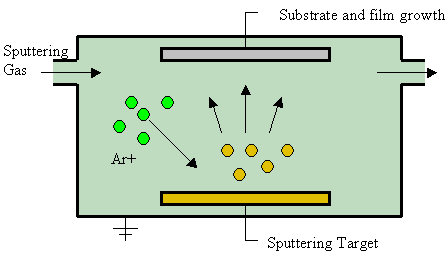
\includegraphics[width=0.4\textwidth]{ch3/sputter}
\caption{Sputtering deposition schematics(\url{https://www.wikiwand.com/en/Sputter_deposition})}
\end{wrapfigure}
After creating the distinct and separate layers for transporting and absorbing parameters we have to create a second contact for the device. 
In our case, the sputtering method PVD is used. It uses a material called a target(an item consisting of a desirable material) from which parts are ejected into the substrate. The sputter gas is pumped into the chamber, where a magnetic and electric fields are both confined. The gas atoms thump target ions which create the plasma in the chamber and then they hit the substrate. 

\begin{figure}[t]
  \centering
  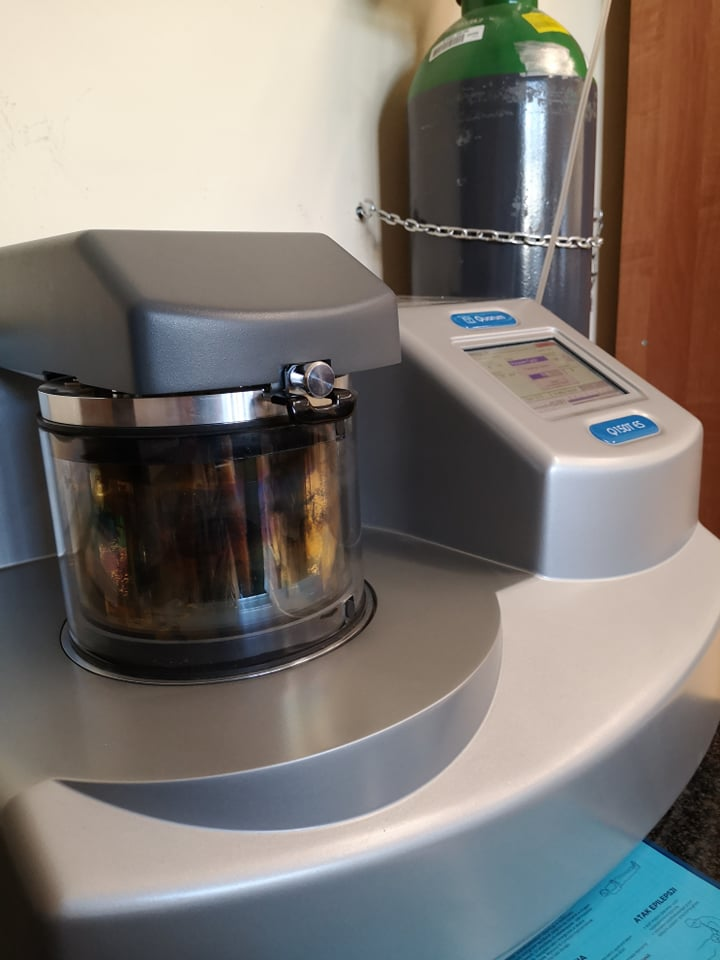
\includegraphics[width=.4\textwidth]{ch3/napylara}  
  \caption{Sputtering deposition device that we were using}
\end{figure}

